\documentclass{article}
% PACKAGES
\usepackage[english]{babel}
\usepackage{graphicx} % Required for inserting images
\usepackage[most]{tcolorbox}
\usepackage{lmodern}
\usepackage{titlepic}
\usepackage{pdfpages}
\usepackage{tcolorbox}
\usepackage{amsmath}
\usepackage{polynom}
\usepackage{pgfplots}
\usepackage{xcolor}
\usepackage{tikz}
\usepackage{color,soul}
\usepackage{enumerate}
\usepackage{enumitem}
\usepackage{cancel}
\usepackage{hyperref} 
\usepackage{tikzsymbols}
\usepackage{fontawesome5}
\usepackage[export]{adjustbox}
\usepackage{amssymb}
\usepackage{tikz,lipsum,lmodern}
\usepackage{booktabs}
\usepackage{tikzsymbols}
\usepackage{textcomp}
\usepackage{marvosym}
\usepackage{parskip}
\usepackage{MnSymbol,wasysym}


% tikz library 
\usetikzlibrary{patterns}

% newcommand 
\newcommand*\circled[1]{\tikz[baseline=(char.base)]{
            \node[shape=circle,draw,inner sep=2pt] (char) {#1};}}
% COLOURS
\definecolor{Orchid}{RGB}{218, 112, 214}
\definecolor{snow}{rgb}{1.0, 0.98, 0.98}
\definecolor{mordantred19}{rgb}{0.68, 0.05, 0.0}
\definecolor{mistyrose}{rgb}{1.0, 0.89, 0.88}
\definecolor{nadeshikopink}{rgb}{0.96, 0.68, 0.78}
\definecolor{cadmiumgreen}{rgb}{0.0, 0.42, 0.24}
\definecolor{OliveGreen}{RGB}{85, 107, 47}
\definecolor{RoyalPurple}{RGB}{120, 81, 169}
\definecolor{NavyBlue}{RGB}{0, 0, 128}
\definecolor{CornflowerBlue}{RGB}{100, 149, 237}
\definecolor{Cerulean}{RGB}{0, 123, 167}
\definecolor{DarkOrchid}{RGB}{153, 50, 204}

\title{MCV4U - Calculus and Vectors [Chapter 4]}
\author{Kensukeken}
\date{April 18th, 2024}

\begin{document}
\maketitle

\tableofcontents
\newpage
\section{Unit 4 - Curve Sketching}
\subsection{Increasing and Decreasing Functions}
For a continuous and differentiable function, f, the function values(y-values) are increasing for all x-values where $f'(x)>0$, and the function values (y-values) are decreasing for all x-values where $f'(c)<0$
\subsubsection{Example 1a)}
Determine the intervals of increase and decrease for the function $$y=x^3+3x^2-2$$
\subsubsection*{Solution:}
\begin{align*}
    y&=3x^2+6x\\
    &=3(x+2)
\end{align*}
\begin{center}
 \begin{tikzpicture}[scale=1.5]
  % Draw axes
  \draw[->] (-3,0) -- (1.5,0) node[right] {$y'$};
  % Draw points
  \filldraw[black] (-2,0) circle (1pt) node[below] {$-2$};
  \filldraw[black] (0,0) circle (1pt) node[below] {$0$};
  
  % Draw plus and minus signs
  \node at (-2.5,0.3) {$+$};
  \node at (-1,0.3) {$-$};
  \node at (1,0.3) {$+$};
\end{tikzpicture}
\end{center}

$\therefore$ the intervals of increase are $x\in(-\infty,-2)\cup(0, \infty)$

$\therefore$ the intervals of decrease are $x\in (-2,0)$

\subsubsection{Example 1b)}
Determine the intervals of increase and decrease of the function $f(x)=\frac{x}{x^2+1}$
\subsubsection*{Solution:}
\begin{align*}
    f'(x)&=\frac{x^2+1(1)-(x)(2x)}{(x^2+1)^2}\\
    &=\frac{x^2+1-2x^2}{(x^2+1)^2}\\
    &=\frac{-x^2+1}{(x^2+1)^2}\\
    &=\frac{-(x^2-1)}{(x^2+1)}\\
    &=\frac{-(x-1)(x+1)}{(x^2+1)^2}
\end{align*}

$\therefore$ the intervals of increase are $x\in(-\infty,-1)\cup(1, \infty)$

$\therefore$ the intervals of decrease are $x\in (-1,1)$
\subsubsection{Example 2}
Given a graph of $y=f'(x)$, graph the curve $y=f(x)$

\begin{center}
\begin{tikzpicture}[scale=0.6]
  % Grid
  \draw[gray!50,very thin] (-2,-2) grid (5,5);
  \draw[thick,->] (-2,0) -- (5,0) node[right] {$x$};
  \draw[thick,->] (0,-2) -- (0,5) node[above] {$y$};
  
  % Plot of f'(x)
  \draw[blue,domain=-0.3:2.3,smooth,variable=\x] plot ({\x},{3*\x*\x - 6*\x + 2}) node[right] {$f'(x)$};
  
  % Fill between curve and x-axis
  \fill[pattern=north east lines,pattern color=gray!50,domain=0:2.26328,variable=\x] (0,0) -- plot ({\x},{3*\x*\x - 6*\x + 2}) -- (3.16228,0) -- cycle;
  
  % Plot of f(x)
  \draw[red,domain=-0.5:2.7,smooth,variable=\x] plot ({\x},{\x*\x*\x - 3*\x*\x + 2*\x + 1}) node[right] {$f(x)$};
\end{tikzpicture}
\end{center}
\subsubsection{Example 3}
Find the constants a, b and c such that the graph of $y=-x^3+ax^2+bx+c$ will decrease to the point (-6, -200) and increase to the point (2, 56) and then decrease thereafter.
\subsubsection*{Solution:}
\begin{align*}
    y'&=-3x^2+2ax+b\\
    f'(-6)=0 &\implies -3(-6)^2+2a(-6)+b=0\\
    &-108-12a+b=0\\
    b&=12a+108 \quad \circled{1}\\
    f'(2)=0 &\implies -3(2)^2+2a(2)+b=0\\
    b&=-4a+12 \quad \circled{2}\\
    12a+108&=-6a+12\\
    16a&=-96\\
    a&=-6\\
    b&=-4a+12\\
    &=-4(-6)+2\\
    b&=36
    y=-x^3-6x^2+36x+c\\
    &\textbf{sub } (-6,-200)\\
    -200&=-(-6)^3-6(-6)^2+36(-6)+c\\
    16&=c \quad \therefore a=-6, b=36, c=16
\end{align*}
\subsection{Critical Points, Local Maxima and Local Minima}
\subsubsection{First Derivative Test:}
If $f'(x)$ goes from positive to 0 to negative, then there is a local maximum at the point where $f'(x)=0$
\begin{center}
\begin{tikzpicture}[scale=1.5]
  % Draw function f'(x)
  \draw[blue, thick, domain=0.5:2.5, smooth, variable=\x] plot ({\x},{-0.6*(\x-1.5)^2 + 1.8}) node[right] {$f'(x)$};
  
  % Draw local maximum point
  \filldraw[red] (1.5,1.8) circle (1pt) node[above right] {Local Maximum};
\end{tikzpicture}
\end{center}

Similarly, if $f'(x)$ goes from positive to undefined to negative, and if $f(x)$ is defined at the point where $f'(x)$ is undefined, then there is a local maximum at the point where $f'(x)=0$

\begin{center}
\begin{tikzpicture}[scale=1,cap=round]
 \tikzset{axes/.style={}}
 % The graphic
\begin{scope}[style=axes]
\draw[->] (-.5,0) -- (3,0) node[below] {$x$};
\draw[->] (0,-.5)-- (0,3) node[left] {$y$};
\draw[thick] (0.25,0.4) to [out=10,in=-90]  (1.5,2.5)
 to [out=-90, in=175] (2.75,.4);
\draw[thin] (1.5,2.5) -- ++ (0.2,0.6) node[above]{$f'(a)$ does not exist};
\draw (1.5,0.2) -- (1.5,-0.2) node[below]{$a$};
\end{scope}
\end{tikzpicture}
\end{center}

If $f'(x)$ goes from negative to 0 to negative, then there is a local minimum at the point where $f'(x)=0$

\begin{center}
\begin{tikzpicture}[scale=1.5]
  % Draw function f'(x)
  \draw[blue, thick, domain=0.5:2.5, smooth, variable=\x] plot ({\x},{0.6*(\x-1.5)^2 + 1.8}) node[right] {$f'(x)$};
  
  % Draw local minimum point
  \filldraw[red] (1.5,1.8) circle (1pt) node[below left] {Local Minimum};
\end{tikzpicture}
\end{center}

Similarly, if $f'(x)$ goes from negative to undefined to positive, and if $f(x)$ is defined at the point where $f'(x)$ is undefined, then there is a local minimum at the point where $f'(x)=0$
\begin{center}
\begin{tikzpicture}[scale=1.2,cap=round]
  % Axes
  \draw[->] (-0.5,0) -- (3,0) node[below] {$x$};
  \draw[->] (0,-0.5)-- (0,3) node[left] {$y$};
  
  % Curve
  \draw[thick] (0.25,2.6) to[out=-10,in=90] (1.5,0.5) to[out=80,in=175] (2.75,2.6);
  
  % Point and label for local minimum
  \draw (1.5,0.2) -- (1.5,-0.2) node[below] {$a$};
  
  % Label for "f'(a) does not exist"
  \draw[thin] (1.5,0.5) -- ++ (0,0.7) node[above, left] {$f'(a)$ does not exist};
\end{tikzpicture}
\end{center}

If $f'(x)$ goes from positive to 0 positive, then there is neither a maximum nor a minimum.
\begin{center}
\begin{tikzpicture}[scale=1.5]
  % Draw axes
  \draw[->] (-2,0) -- (2,0) node[right] {$x$};
  \draw[->] (0,-2) -- (0,2) node[above] {$y$};
  
  % Plot of x^3
  \draw[blue, thick, domain=-1:1.1, smooth, variable=\x] plot ({\x},{\x*\x*\x}) node[right] {$f(x)=x^3$};
  
  % Label indicating positive slope
  \node[above right] at (1,2) {Positive slope};  
  % Label indicating positive slope again
  \node[below left] at (-1,-1) {Positive slope};
\end{tikzpicture}
\end{center}
If $f'(x)$ goes from negative to 0 negative, then there is neither a maximum nor a minimum.
\begin{center}
\begin{tikzpicture}[scale=1.5]
  % Draw axes
  \draw[->] (-2,0) -- (2,0) node[right] {$x$};
  \draw[->] (0,-2) -- (0,2) node[above] {$y$};
  
  % Plot of x^-3 (negative part)
 \draw[blue, thick, domain=-1:1.1, smooth, variable=\x] plot (-{\x},{\x*\x*\x}) node[left] {$f(x)=-x^3$};
  
  % Label indicating negative slope
  \node[above left] at (-1,2) {Negative slope};
  
  % Label indicating negative slope again
  \node[below right] at (1,-1) {Negative slope};
\end{tikzpicture}
\end{center}
\subsubsection{Critical Points and Critical Numbers}
The points at which $f(x)$ is defined and $f'(x)$ is undefined are called critical points.

The values of x at which $f'(x)=0$ or $f'(x)$ is undefined are called critical numbers.

\subsubsection{Example 1}
For function $y=x^4-8x^3+18x^2$, determine all critical points. Determine whether each of these values of x gives a local maximum or neither.
\subsubsection*{Solution:}
\begin{align*}
    y'=4x^3-24x^2+36x\\
    &=4x(x^2-6x+9)\\
    &=4x(x-3)^2
\end{align*}
Our critical numbers are $x=0$ and $x=3$\\
\begin{align*}
    &\text{at } x=0, y=(0)^4-8(0)^3+18(0)^2\\
    &(0,0)\\
    &\text{at } x=3, y=(3)^4-8(3)^3+18(3)^2\\
    &(3,27)
\end{align*}
$\therefore$ Our critical points are (0,0) which represents a minimum and (3,27) which represents neither a minimum nor a maximum.
\subsubsection{Example 2}
Determine whether the function $f(x)=x^3$ has a maximum or a minimum or neither at $(c, f(c))$ where $f'(c)=c.$
\subsubsection*{Solution}
\begin{align*}
    f'(x)&=3x^2\\
    3x^2=0 &\implies x=0\\
    \text{at } x=0,& y=(0)^3\\
    &=0\\
    &(0,0)
\end{align*}
$\therefore$ at (0,0) there is neither a maximum nor a minimum.

\newpage
\subsection{Asymptotes etc.}
\subsubsection{Testing for Vertical Asymptotes and Holes} 
Given a rational function of the form $$f(x)=\frac{p(x)}{q(x)},$$ we should simplify by crossing out like factors from the numerator and the denominator. 
\begin{enumerate}
    \item There is a hole at $x = c$ if the factor $(x –c)$ was originally present in both the numerator and the denominator and if the degree of that factor in the numerator was greater than or equal to the degree of that factor in the denominator. In other words, if $(x –c)$ is present in both the numerator and denominator and if, after simplifying, it is completely crossed out of the denominator, then there is a hole at  $x = c$. To determine the y-coordinate of the hole, plug the x-value into the simplified rational expression.
    \item There’s a vertical asymptote at $x = c$ if, AFTER SIMPLIFYING, the denominator equals 0 at $x = c$ and the numerator does not equal 0at $x = c$.
\end{enumerate}

\subsubsection{Test for Horizontal and Oblique Asymptotes}
Given a rational function of the form $$f(x)=\frac{p(x)}{q(x)},$$ we should simplify by crossing out like factors from the numerator and the denominator. If the denominator is degree 0 (i.e, there are no more x’s), then there are no horizontal or oblique asymptotes. If the denominator is not degree 0, then, AFTER SIMPLIFYING:
\begin{enumerate}
    \item There’s a horizontal asymptote at y = 0 if the degree of the denominator is greater than the degree of the numerator.
    \item There’s a horizontal asymptote at $$y=\frac{\text{lead coefficient of numerator}}{\text{lead coefficient of denominator}}$$ if the degree of the numerator equals the degree of the denominator. (Remember, the denominator must be at least degree 1 after simplifying)
    \item There’s an oblique asymptote if the degree of the numerator is greater than the degree of the denominator.  To determine the equation of the oblique asymptote, we use synthetic division or long division
\end{enumerate}
\subsubsection{Example 1}
Determine the equation of any asymptotes and the location of any holes(including y-coordinates) of the function $y=\frac{2x-2}{x^2+3x-4}$
\subsubsection*{Solution}
\begin{align*}
    &=\frac{2(x-1)}{(x+4)(x-1)}\\
    &=\frac{2}{(x+4)}\\
    &\text{hole at } x=1\\
    &\text{y-coordinate of hole: } \frac{2}{1+4}=\frac{2}{5}\\
    &\text{hole at } \left(1, \frac{2}{5}\right)\\
    &\text{V.A at } x=-4\\
    &\frac{\text{degree 1}}{\text{degree 2}} \implies \text{H.A at } y=0
\end{align*}
\subsubsection{Example 2}
Determine the equations of any asymptotes and the locations of any holes(including y-coordinate) of the function $y=\frac{5x+15}{2x+12}$
\subsubsection*{Solution}
\begin{align*}
    &y=\frac{5(x+3)}{2(x+6)}\\
    & \text{V.A at } x=-6\\
    & \text{H.A at } y=\frac{5}{2}
\end{align*}
\subsubsection{Example 3}
Determine the equations of any asymptotes and the locations of any holes(including y-coordinate) of the function $y=\frac{3x^2+15x-18}{4x^2-20x-24}$
\subsubsection*{Solution}
\begin{align*}
    &=\frac{3(x+6)(x-1)}{4(x-6)(x+1)}\\
    &\text{V.A at } x=6 \text{ and } x=-1\\
    &\text{H.A at } y=\frac{3}{4}
\end{align*}
\subsubsection{Example 4}
Determine the equation of any asymptotes and the location of any holes(including y-coordinate) of the function $y=\frac{x^2-2x+4}{x-3}$
\subsubsection*{Solution}
We cannot factor
$\therefore$ V.A at x=3\\
oblique (or slant) aspmptote 
$$\polyhornerscheme[x=3]{x^2-2x+4}$$
$$y=x+1+\frac{7}{x-3}$$
$$\therefore \text{O.A at } y=x+1$$
\subsubsection{Example 5}
Find constants a and b such that the graph of the function $y=\frac{ax+8}{bx-1}$ has a horizontal asymptote at $y=8$ and a vertical asymptote at $x=-5$
\subsubsection*{Solution}
\begin{align*}
    \text{V.A at } x=-5 \implies b(-5)-1&=0\\
    -5b-1&=0\\
    -5b&=1\\
    b&=-\frac{1}{5}\\
    \text{H.A at } y=8 \implies \frac{a}{b}&=8\\
    \frac{a}{-\frac{1}{5}}=8 \implies a &=-\frac{8}{5}\\
    \therefore a=-\frac{8}{5}, \quad b&=-\frac{1}{5}
\end{align*}
\newpage
\subsection{Concavity and Points of Inflection}
\subsubsection{Concave Up [$f''(x)>0$]}
\underline{Concave Up:} $f''(x)>0$. The graph of $y=f(x)$ is a concave up when the second derivative is positive. i.e when $f''(x)>0$.
\begin{figure}[ht]
    \centering
    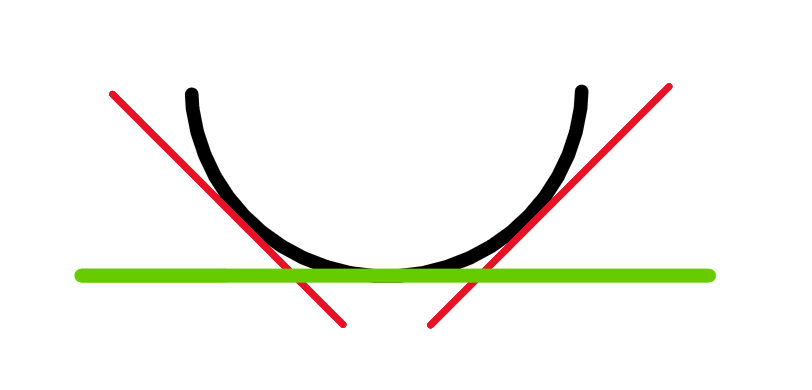
\includegraphics[width=0.7\textwidth]{imgs/concave-up.png}
\end{figure}

Notice that the tangent lines go from a slope of negative to zero to positive. In other words the slopes are increasing meaning that the rate of change of the rate of change is positive(i.e $f''(x)>0$). When $f''(x)>0$, the curve is above the tangent lines. 

\subsubsection{Concave Down [$f''(x)<0$]}
\underline{Concave Down: } $f''(x)<0$. The graph of $y=f(x)$ is concave down when the second derivative is negative. i.e, when $f''(x)<0$.
\begin{figure}[ht]
    \centering
    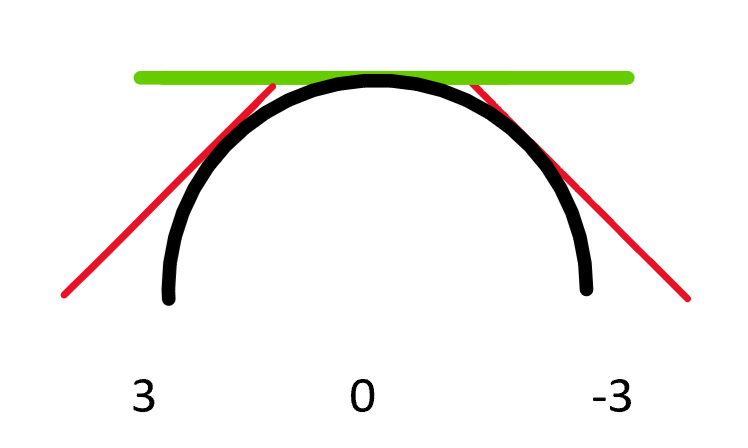
\includegraphics[width=0.7\textwidth]{imgs/concave-down.png}
\end{figure}

Notice that the tangent lines go from a slope of positive,to zero, to negative. In other words, the slopes are decreasing, meaning that the rate of change of the rate of change is negative (i.e  $f''(x)<0$). When $f''(x)<0$, the curve is below the tangent lines.

\subsubsection{Second Derivative Test}
If at a given point, $f'(x)=0$ and $f''(x)=0$, then there is a local minimum.
\begin{figure}[ht]
    \centering
    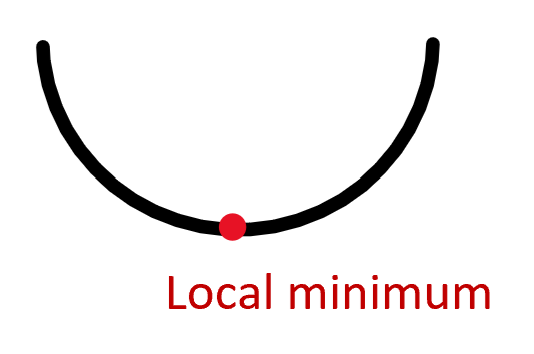
\includegraphics[width=0.5\textwidth]{imgs/local-minimum.png}
\end{figure}

If at a given point, $f'(x)=0$ and $f''(x)<0$, then there is a local maximum.
\begin{figure}[ht]
    \centering
    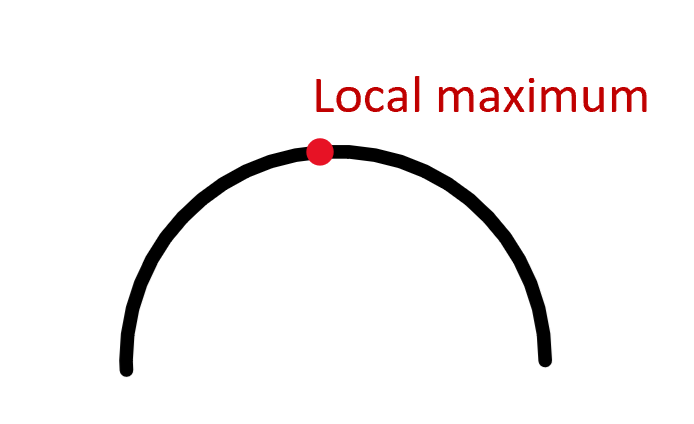
\includegraphics[width=0.5\textwidth]{imgs/local-maximum.png}
\end{figure}

\subsubsection{Points of Inflections}
Points at which $f''(x)=0$ are called points of inflection.
\begin{figure}[ht]
    \centering
    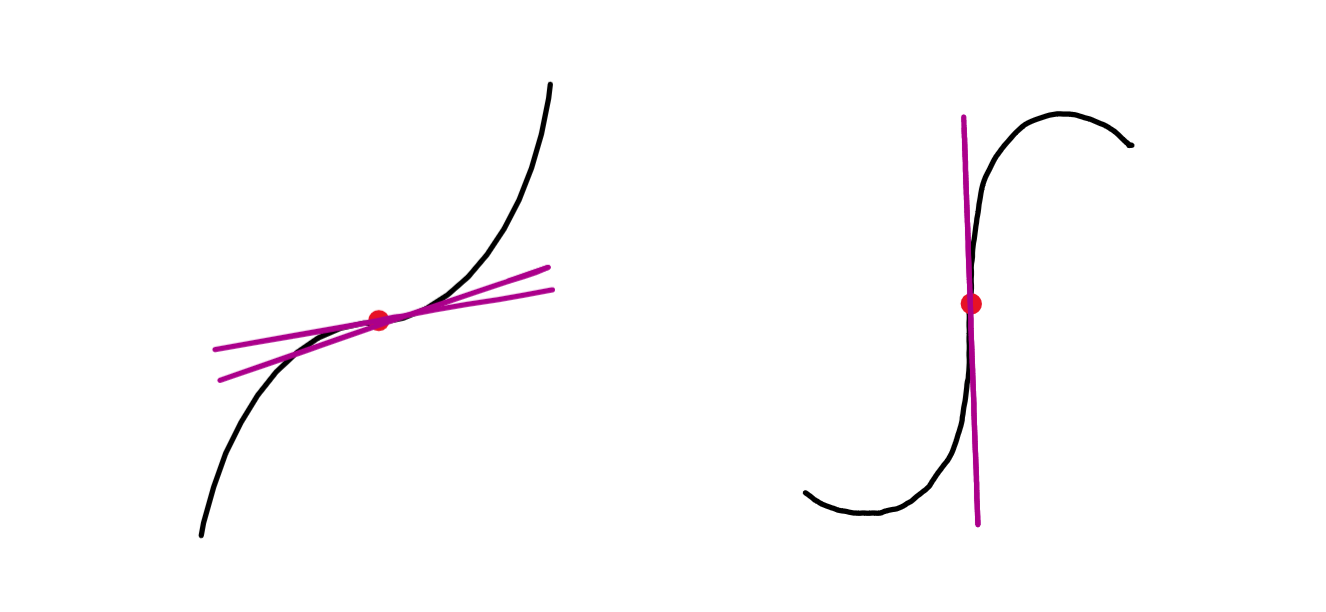
\includegraphics[width=0.7\textwidth]{imgs/points_of_inflections.png}
\end{figure}
\newpage 
\subsubsection{Putting Together $f'(x)$ and $f''(x)$}

\begin{figure}[h]
    \centering
    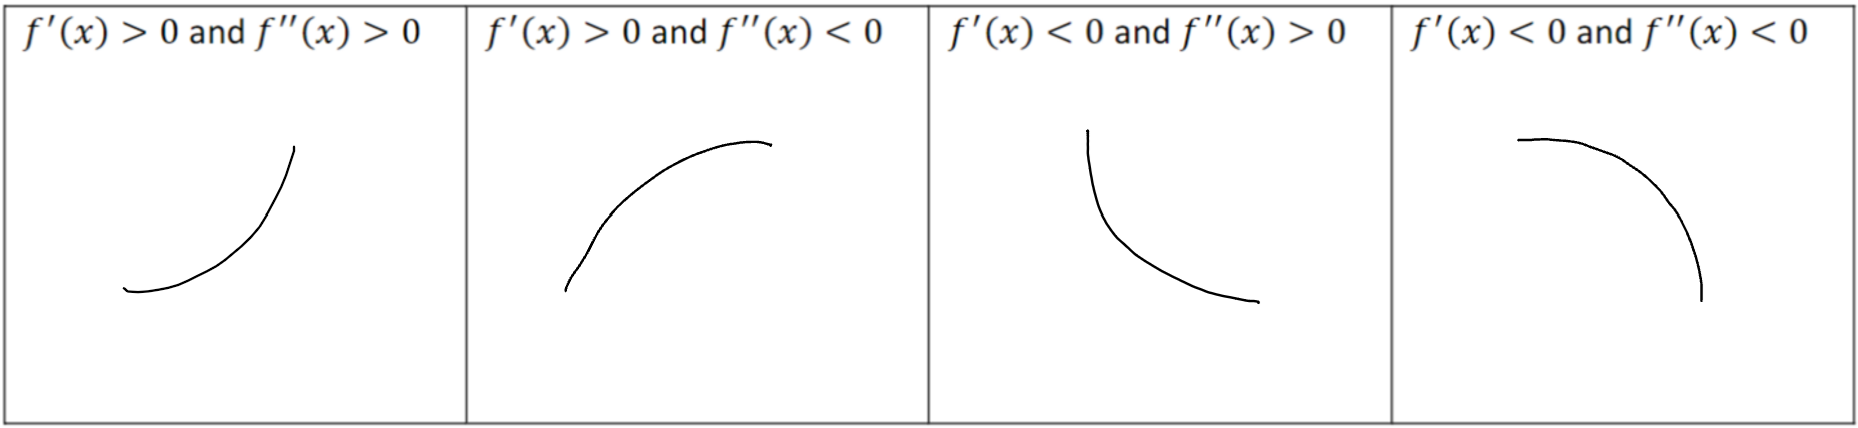
\includegraphics[width=1\textwidth]{imgs/putting_together.png}
\end{figure}
\subsubsection{Key Ideas}
\textbf{Concavity:}
\begin{itemize}
    \item The graph of a function is concave up on an interval if it is increasing on the interval.
    \item The graph of a function is concave down on an interval if it is decreasing on the interval.
\end{itemize}

\textbf{Point of Inflection:}
\begin{itemize}
    \item A point of inflection is a point on the graph of a function where the function changes from concave up to concave down, or vice versa, or is undefined if it is a point of inflection on the graph.
\end{itemize}

\textbf{Need to Know:}
\begin{itemize}
    \item Test for concavity: If $f$ is a differentiable function whose second derivative exists on an open interval $I$, then
    \begin{itemize}
        \item the graph of $f$ is concave up on $I$ if $f''(x) > 0$ for all values of $x$ in $I$.
        \item the graph of $f$ is concave down on $I$ if $f''(x) < 0$ for all values of $x$ in $I$.
    \end{itemize}
    \item The second derivative test: Suppose that $f$ is a function for which $f'(c) = 0$ and the second derivative $f''(x)$ exists on an interval containing $c$.
    \begin{itemize}
        \item If $f''(c) > 0$, then $f$ has a local minimum value at $x = c$.
        \item If $f''(c) < 0$, then $f$ has a local maximum value at $x = c$.
        \item If $f''(c) = 0$, then the test fails. Use the first derivative test.
    \end{itemize}
\end{itemize}
\newpage
\subsection*{Example 1}
Sketch the graph of $y=x^3-3x^2-9x+10$
\subsection*{Solution}
\begin{align*}
    y' &= 3x - 6x - 9 \\
    &= 3(x^2 - 2x - 3) \\
    &= 3(x - 3)(x + 1) \\
    y' &= 3(x - 3)(x + 1) \\
    y' = 0 & \text{ at } x = 3 \text{ and } x = -1
\end{align*}
\begin{minipage}{0.5\linewidth}
At $x=-3$ 
\begin{align*}
    y&=3^3-3(3)^2-9(3)+10\\
    &=-17\\
    &(3,-17)
\end{align*}
\end{minipage}
\begin{minipage}{0.5\linewidth}
At $x=-1$ 
\begin{align*}
    y&=(-1)^3-3(-1)^2-9(-1)+10\\
    &=15\\
    &(-1,15)
\end{align*}
\end{minipage}
\begin{minipage}{0.5\linewidth}
\begin{align*}
    y'' &= 6x - 6 \\
    &= 6(x - 1) \\
    y'' &= 0 \quad \text{at } x = 1
\end{align*}
\end{minipage}
\begin{minipage}{0.5\linewidth}
\begin{align*}
\text{At } x &= 1 \\
y &= (1)^3 - 3(1)^2 - 9(1) + 10 \\
&= -1 \\
&(1, -1)
\end{align*}
\end{minipage}
\begin{figure}[h]
    \centering
    \begin{minipage}{0.5\textwidth}
        \centering
        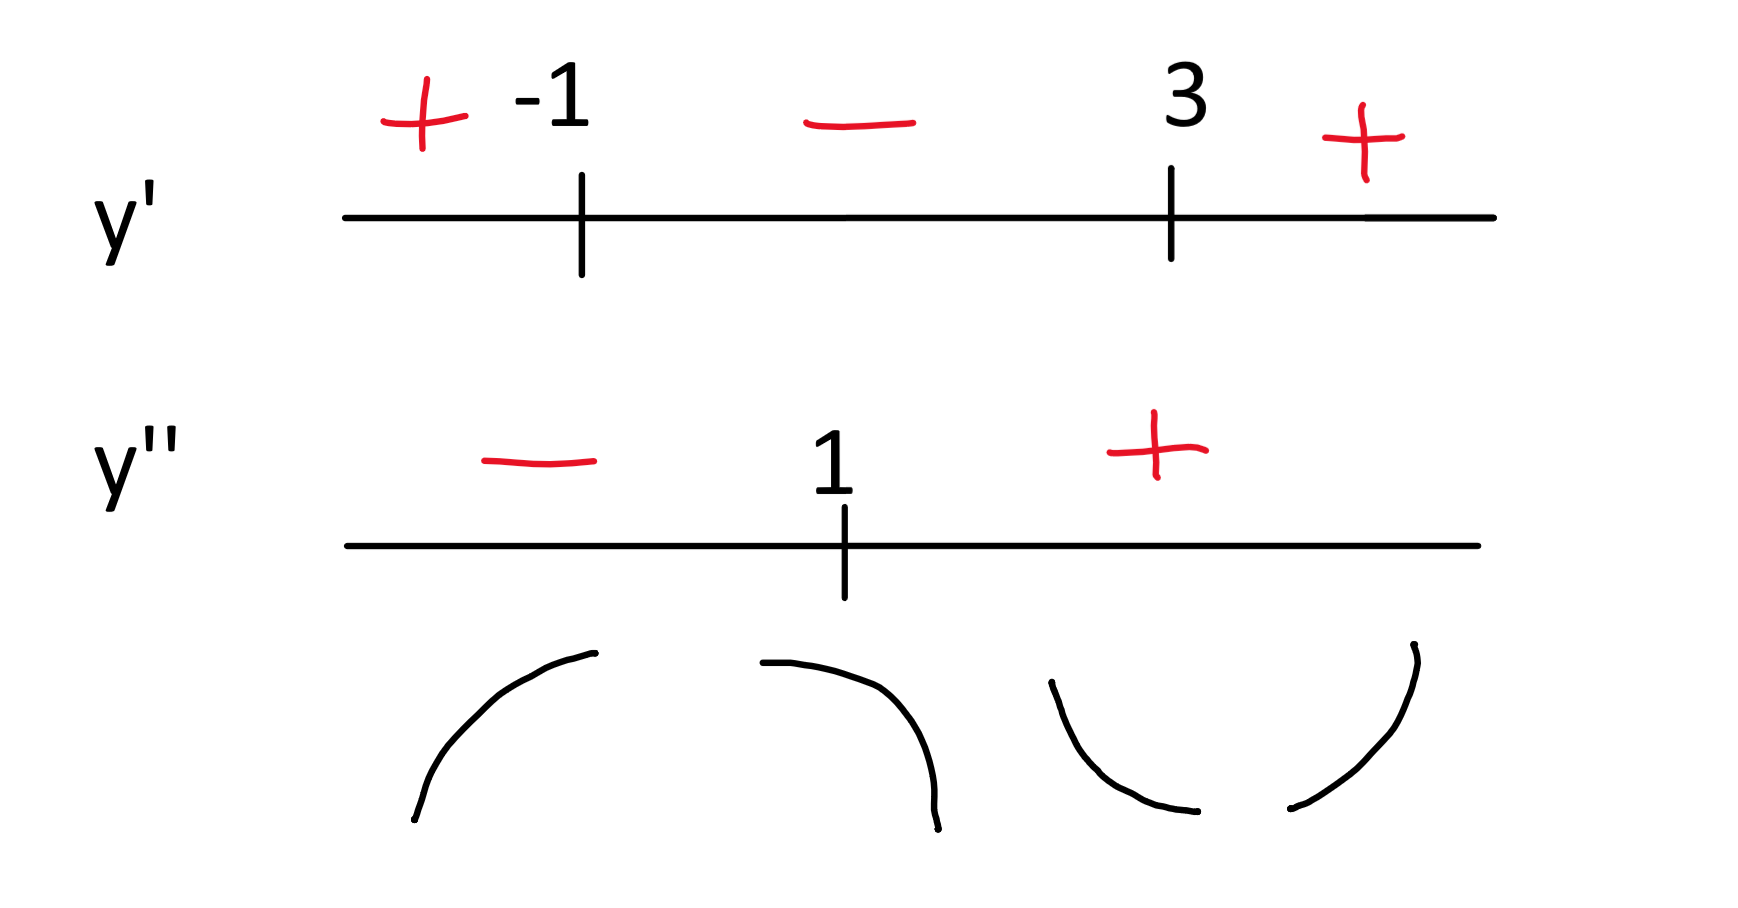
\includegraphics[width=\textwidth]{imgs/alg 1.png}
        \caption{Intervals}
        \label{fig:alg1}
    \end{minipage}%
    \begin{minipage}{0.5\textwidth}
        \centering
        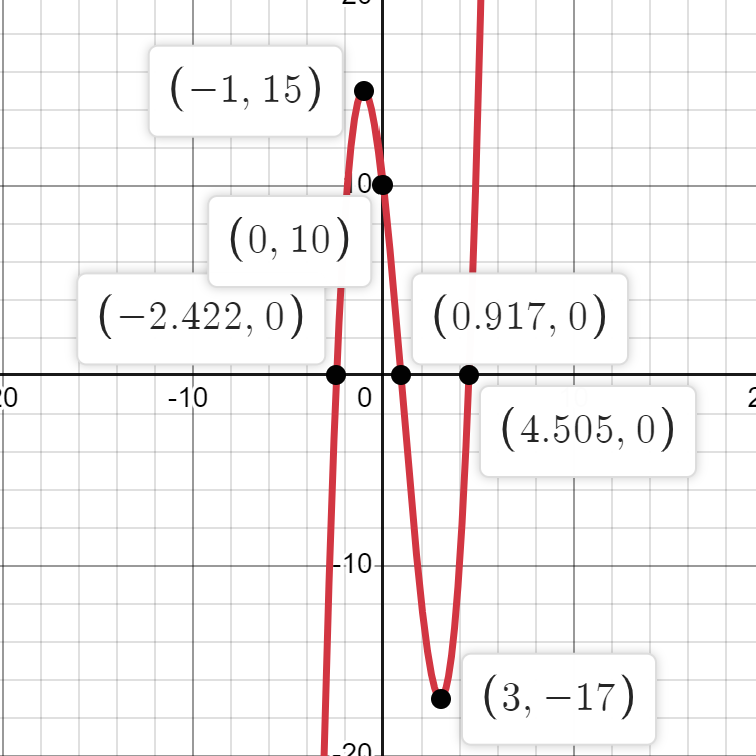
\includegraphics[width=\textwidth]{imgs/y=x^3-3x^2-9x+10.png}
        \caption{Graph of $y=x^3-3x^2-9x+10$}
        \label{fig:graph}
    \end{minipage}
\end{figure}
\newpage 
\subsection*{Example 2}
Sketch the graph of the function $f(x)=x^{\frac{1}{3}}$.
\subsubsection*{Solution}
\begin{align*}
    f'(x)&=\frac{1}{3}x^{-\frac{2}{3}} = \frac{1}{3x^{\frac{2}{3}}}\\
    f''(x)&=-\frac{2}{9}x^{\frac{-5}{3}}=\frac{1}{9x^{\frac{5}{3}}}
\end{align*}
\begin{itemize}
    \item $f'(x)$ never equal 0
    \item $f'(x)$ undefined at $x=0$ (0,0)
    \item $f''(x)$ never equal 0
    \item $f''(x)$ undefined at $x=0$ (0,0)
\end{itemize}
\begin{figure}[h]
    \centering
    \begin{minipage}{0.5\textwidth}
        \centering
        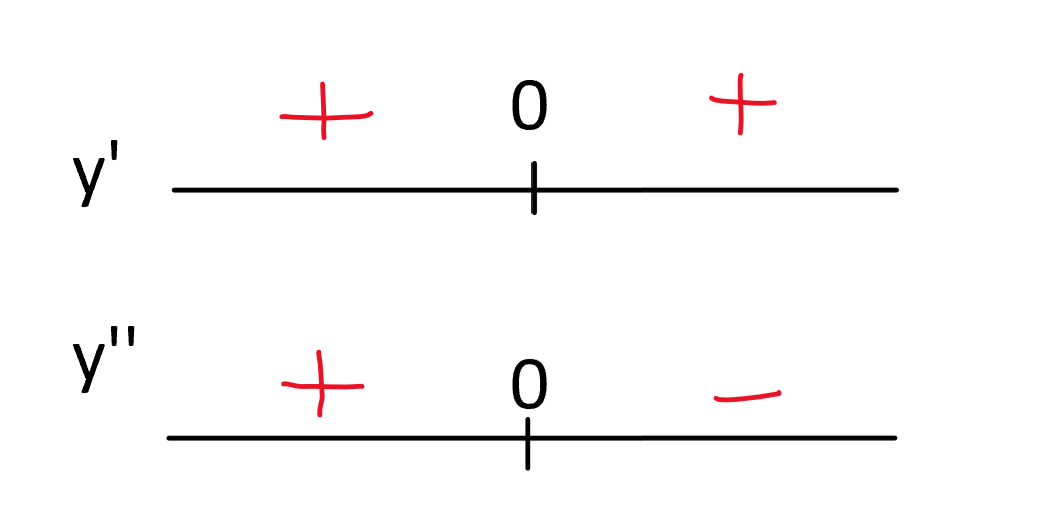
\includegraphics[width=\textwidth]{imgs/alg 2.png}
        \caption{Intervals}
        \label{fig:alg1}
    \end{minipage}%
    \begin{minipage}{0.5\textwidth}
        \centering
        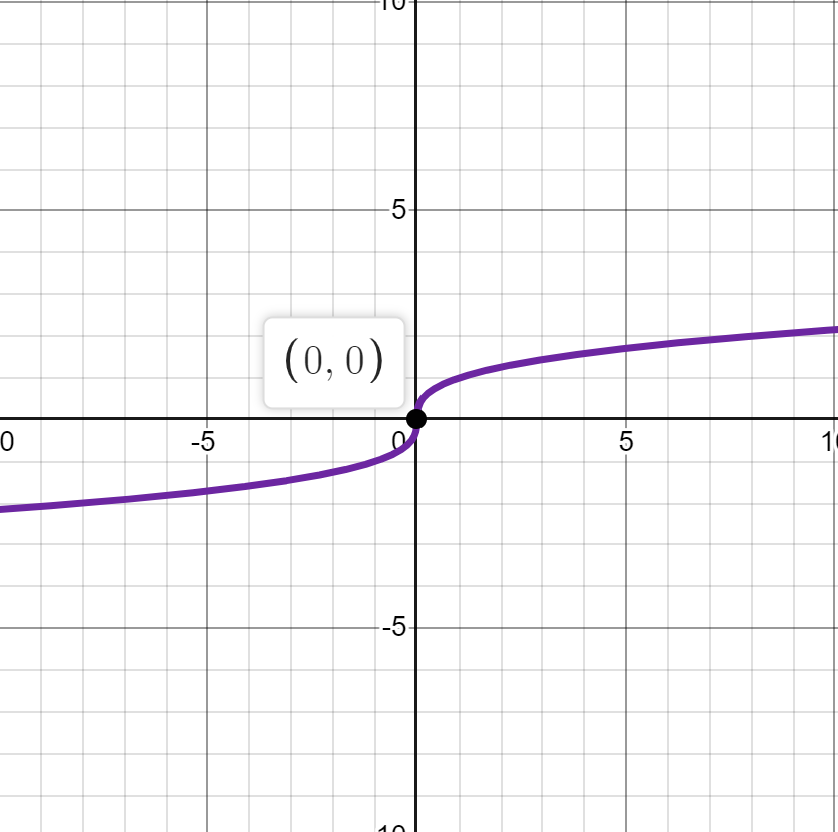
\includegraphics[width=\textwidth]{imgs/y=x^1.png}
        \caption{Graph of $y=x^{\frac{1}{3}}$}
        \label{fig:graph}
    \end{minipage}
\end{figure}
\newpage 
\subsubsection*{Example 3}
Determine any points of inflection on the graph of $f(x)=\frac{1}{x^2+3}$.
\subsubsection*{Solution}
\textbf{First Derivative:}
\begin{align*}
f(x) &= \frac{1}{x^2+3} \\
f'(x) &= \frac{d}{dx} \left(\frac{1}{x^2+3}\right) \\
     &= \frac{0 \cdot (x^2+3) - 1 \cdot 2x}{(x^2+3)^2} \\
     &= \frac{-2x}{(x^2+3)^2}
\end{align*}

\textbf{Second Derivative:}
\begin{align*}
f'(x) &= \frac{-2x}{(x^2+3)^2} \\
f''(x) &= \frac{d}{dx} \left(\frac{-2x}{(x^2+3)^2}\right) \\
      &= \frac{-2(x^2+3)^2 - (-2x) \cdot 2(x^2+3)(2x)}{(x^2+3)^4} \\
      &= \frac{-2(x^4 + 6x^2 + 9) + 8x^2(x^2+3)}{(x^2+3)^4} \\
      &= \frac{-2x^4 - 12x^2 - 18 + 8x^4 + 24x^2}{(x^2+3)^4} \\
      &= \frac{6x^4 + 12x^2 - 18}{(x^2+3)^4}\\
      &=\frac{6(x-1)(x+1)}{(x^+3)^3}
\end{align*}
At $x=-1$
$$y=\frac{1}{(1)^+3}=\frac{1}{4} \quad \left(-1, \frac{1}{4}\right)$$
At $x=1$
$$y=\frac{1}{(-1)^+3}=\frac{1}{4} \quad \left(1, \frac{1}{4}\right)$$
$\therefore$ 2 points of inflection are $$\left(-1, \frac{1}{4}\right) \& \left(1, \frac{1}{4}\right)$$

\subsection{Graphing Curves}
\underline{Algorithm for Curve Sketching:}
\begin{enumerate}
    \item Determine $y$-intercept if it exists (let $x=0$)
    \item Determine $x$-intercepts if they exist (let $y=0$)
    \item Determine any holes (including $y$-coordinate) or vertical asymptotes
    \item Determine any horizontal or oblique asymptotes
    \item Determine intervals of increase and decrease (determine $x$-values at which $y'$ is zero or undefined and do interval testing)
    \item Determine intervals of concavity (determine $x$-values at which $y''$ is zero or undefined and do interval testing)
    \item "Stack" the intervals created in numbers 5 and 6
    \item Determine the associated $y$-values of any points where $y'$ or $y''$ is zero or undefined and graph those points
    \item Don't forget what you already know about graphs \smiley{} 
\end{enumerate}

For the following diagrams, assume that the function is defined all the way through the interval.
\begin{figure}[h]
    \centering
    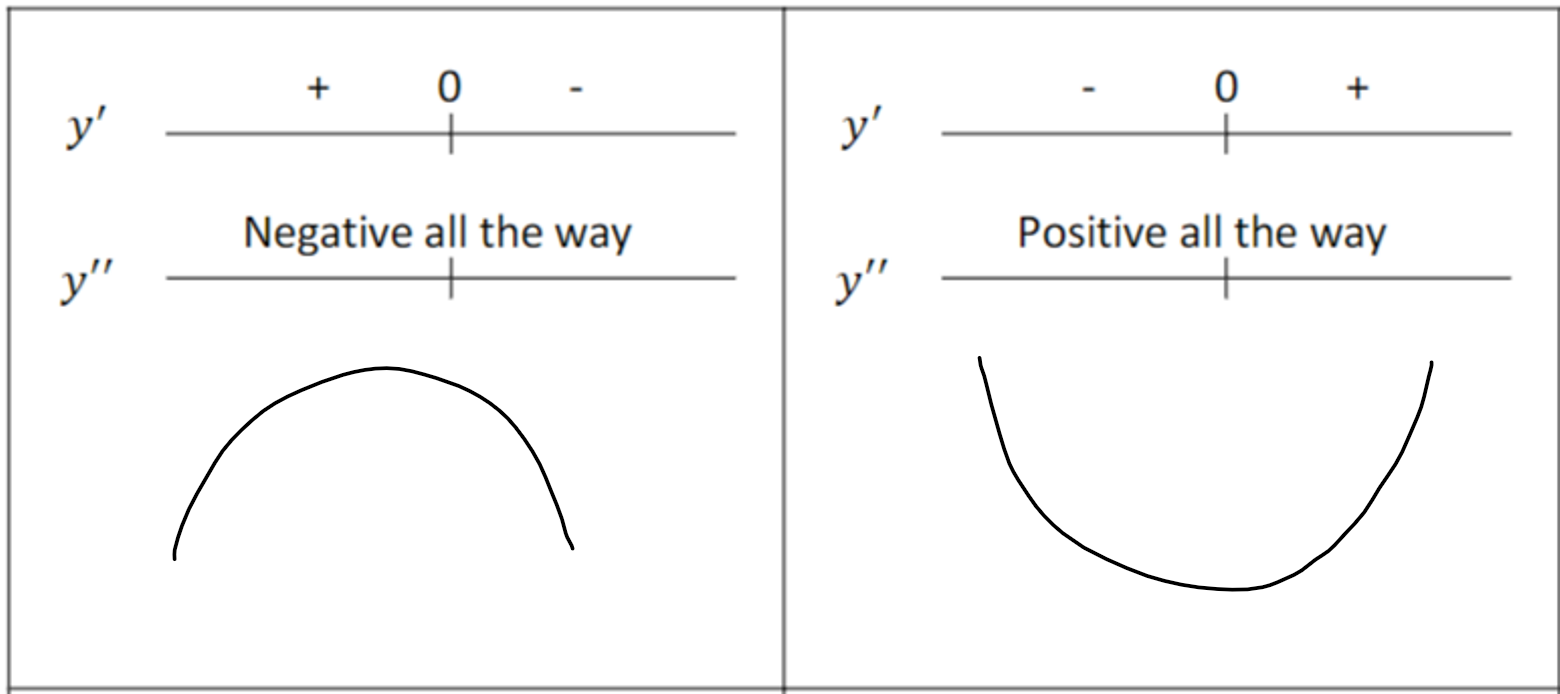
\includegraphics[width=0.9\textwidth]{imgs/diagram_1_2.png}
\end{figure}
\begin{figure}[h]
    \centering
    \begin{minipage}{0.45\textwidth}
        \centering
        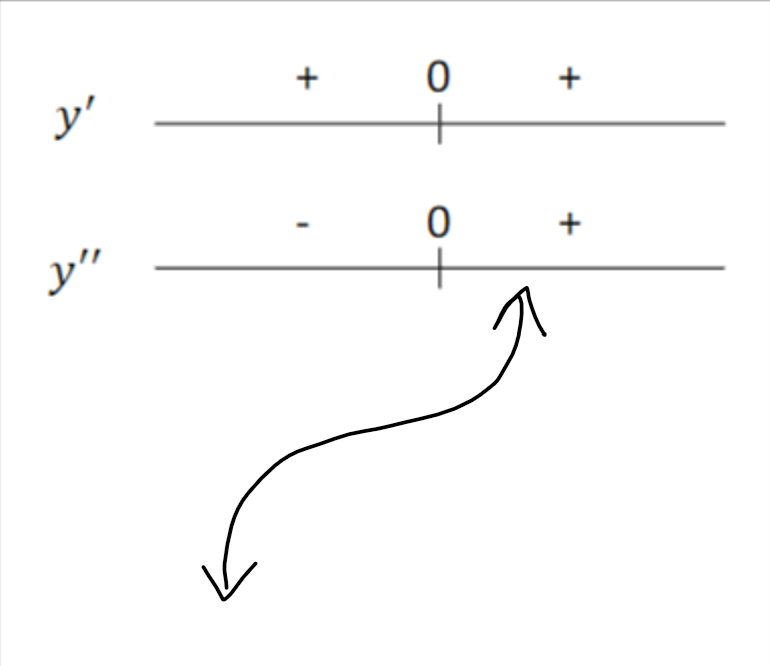
\includegraphics[width=\linewidth]{imgs/diagram_3.png}
    \end{minipage}\hfill
    \begin{minipage}{0.45\textwidth}
        \centering
        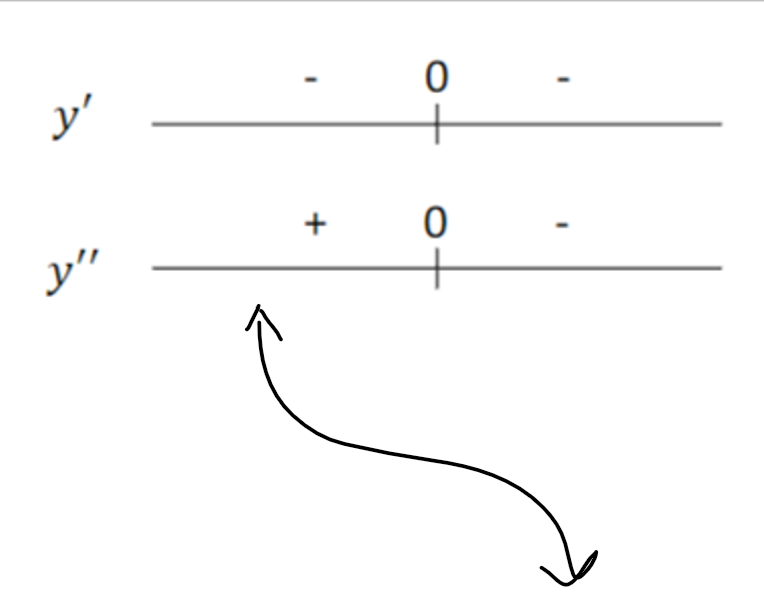
\includegraphics[width=\linewidth]{imgs/diagram_4.png}
    \end{minipage}
\end{figure}
\begin{figure}[h]
    \centering
    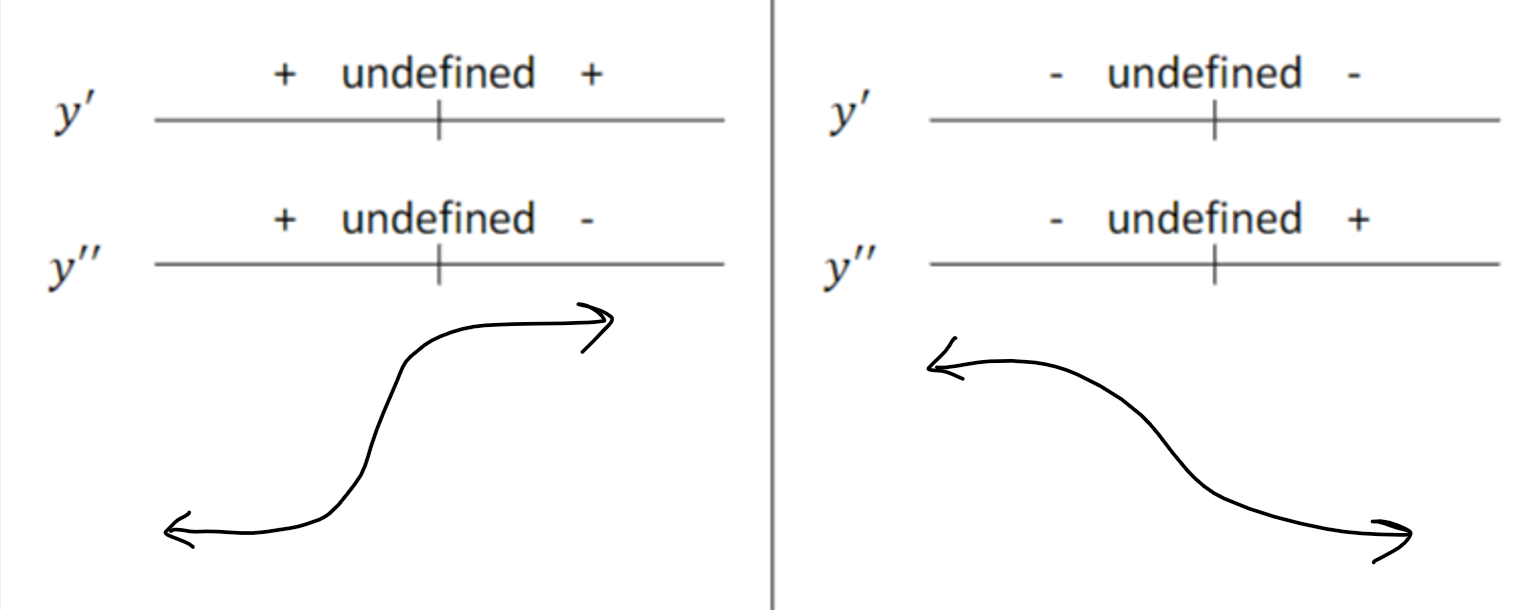
\includegraphics[width=0.9\textwidth]{imgs/diagram_5_6.png}
\end{figure}
\begin{figure}[h]
    \centering
    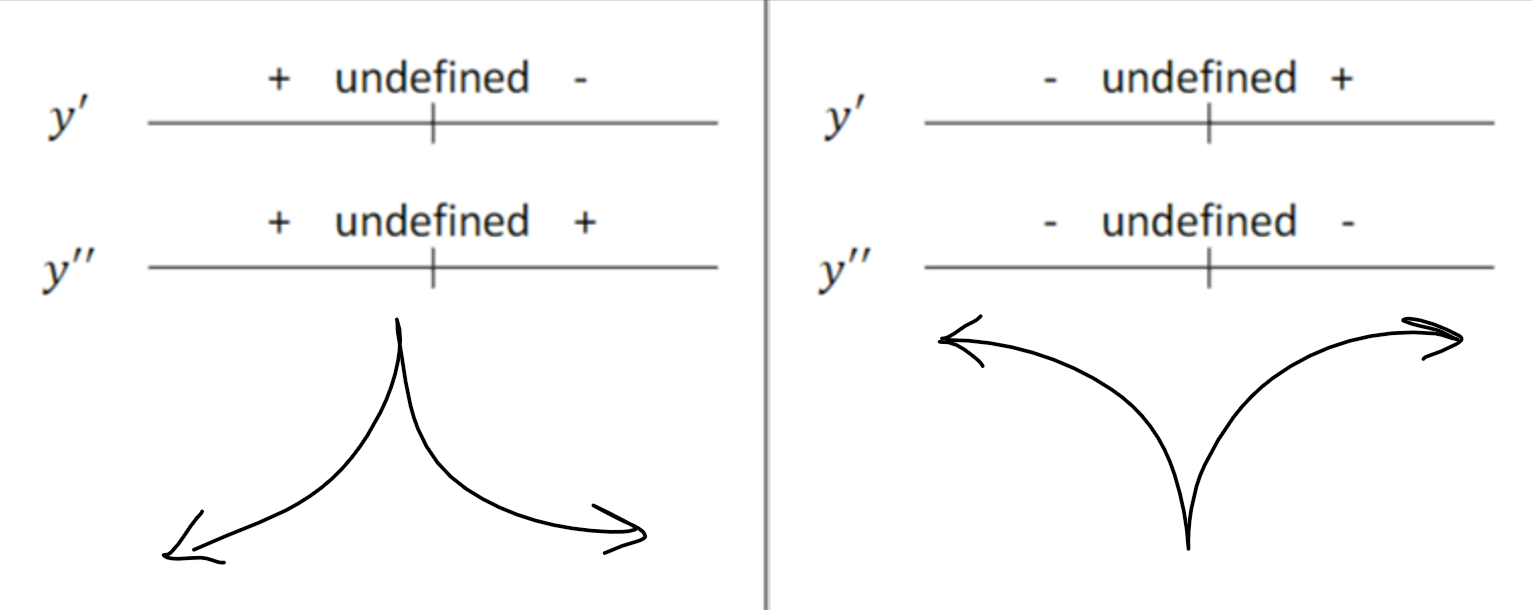
\includegraphics[width=0.9\textwidth]{imgs/diagram_7_8.png}
\end{figure}
\end{document}